\chapter{مقدمه}
در این فصل به معرفی صنعت حمل و نقل درون‌شهری پرداخته می‌شود و ۳ مطالعه موردی از آن با جزئیات بیشتری مورد بررسی قرار خواهند گرفت. در ادامه در فصل‌های بعد به بررسی نیازهای غیر عملکردی  این ۳ مطالعه موردی پرداخته می‌شود. ترتیب و محتوای ارائه این نیازهای غیر عملکردی بر اساس کتاب \cite{bass2003software} انتخاب شده است.

\section{معرفی صنعت حمل و نقل درون شهری}
برای چندین دهه ، برنامه ریزی و حمل و نقل شهری در اطراف خودرو شخصی تکامل یافته است که منجر به مشکلاتی از جمله ازدحام ، صدا ، آلودگی و غیره شده است. همانطور که وارد دهه جدیدی می شویم، تحول دیجیتال همچنان باعث رشد صنعت می شود. معرفی فن آوری های نوظهور و فرآیندهای تجاری، شیوه لجستیک\LTRfootnote{Logestic} و حمل و نقل را تغییر ساختار داده است و این روند احتمالاً در سال های آتی نیز ادامه خواهد داشت ، خصوصاً که نوآوری در فن آوری منجر به رشد پایدار خواهد شد.

صنعت حمل و نقل امروزه همانند زنجیر صنایع مختلف را بهم متصل می کند؛‌شرکت ها و سازمان های بزرگی بر پایه ی پیشرفت های اخیر صنعت حمل‌و‌نقل فرصت ظهور و خودنمایی پیدا کرده اند و سازمان های بزرگی نظیر Uber در آمریکا، OLA cab در هند و DiDi در چین فراتر از مرز های ملی ظاهر شده و در سراسر جهان شروع به ارائه ی خدمات نموده اند.

در این فصل ابتدا به تاکسی‌رانی آنلاین و سهم آن از حمل‌و‌نقل عمومی از کل صنعت حمل‌و‌نقل عمومی درون شهری خواهیم پرداخت؛سپس روش های اشتراک خودرو\LTRfootnote{CarPool} که به تازگی در حال پیدا کردن جایگاه خود در صنعت حمل‌و‌نقل هستند را مورد بررسی قرار خواهیم داد و در پایان این فصل پیرامون یکی از محیط ترین زیرساخت های شهری یعنی پارکینگ های عمومی و ارتباط آن ها به عنوان یک زیرساخت شهری با صنعت حمل‌و‌نقل عمومی درون شهری صحبت خواهیم کرد.
\section{تاکسی‌رانی و حمل‌و‌نقل درون شهری}
تاکسی‌رانی برخط \LTRfootnote{Ride sharing} امروزه در بسیاری از کشور ها سهم زیادی از بازار را در اختیار خود گرفته اند؛برای مثال Uber تا کنون فعالیت خود را به ۷۰ کشور گسترش داده است و میلیون ها راننده برای این غول بزرگ حمل‌و‌نقل درون شهری فعالیت می کنند و روزانه میلیون ها سفر درون شهری بر بستر این شرکت انجام می شود.

شاید استفاده ی راحت مهم ترین نیازی باشد که شرکت هایی نظیر Uber به آن پاسخ داده اند؛تنها کافی است برنامه ای را بر روی تلفن همراه خود نصب داشته باشید و در کمتر از چند دقیقه نزدیک ترین راننده در حال حرکت به سمت شما برای خدمت رسانی خواهد بود.همچنین راه حل هایی که این شرکت ها در زمینه ی پرداخت هزینه ی سفر،‌تضمین امنیت سفر و کاهش هزینه های سفر ارائه داده اند بر استقبال هر چه بیشتر جامعه از این پلتفرم \LTRfootnote{Platform} های تاکسی برخط\LTRfootnote{Online} افزوده است.

در کنار Uber ، از برنامه های جهانی تاکسی‌رانی برخط می توان به DiDi که عمده فعالیت آن در چین است و هچنین \lr{OLA cab} که در هند فعالیت می کند اشاره کرد.

یکی از موارد مطالعه در این پژوهش، پروژه MyWay است.\lr{MyWay} یک پلتفرم مدیریت منابع در صنعت حمل‌و‌نقل هوشمند در شهر های اروپایی است.هدف این پروژه این است که به طور یکپارچه به ادغام کارآمد و منسجم  سرویسهای حمل‌و‌نقل مکمل، در کل زنجیره سفر های درون شهری بپردازد.
MyWay
یک اپ عمومی در حوزه حمل و نقل است تلاش کرده که چندین ویژگی در رابطه تاکسی‌رانی آنلاین، اشتراک‌گذاری خودرو یا استفاده از اتوبوس را در کنار هم برای برنامه‌ریزی سفر استفاده کند که بیشتر در این گزارش ما بر روی قسمت تاکسی‌رانی آنلاین آن تمرکز می‌کنیم.

در پایان این بخش لازم است به این نکته اشاره شود که با ورود شرکت های بزرگ تاکسی‌رانی آنلاین به شهر ها، کسب‌و‌کار های حمل‌و‌نقل سنتی آسیب می بینند و همچنین استفاده از وسایل حمل‌و‌نقل عمومی نیز کاهش خواهد یافت که آثار مخرب زیست محیطی و اجتماعی از جمله معایب گسترش این سیستم هاست.

\subsection{نیازهای عملکردی \lr{Uber}}

مهمترین نیازهای عملکردی در اپ Uber را می‌توان به شرح زیر داشت:

\begin{itemize}
\item 
کاربران باید بتوانند با نام و شماره تلفن و زبان مورد نظر ثبت نام کنند در شکل \ref{fig: uber1} روند این ثبت نام نشان داده شده است که یک SMS برای تایید به شماره تلفنفرستاده می‌شود و سپس نحوه پرداخت پیشنهادی انتخاب می‌شود.
\end{itemize}

\begin{figure}[htb]
\centering
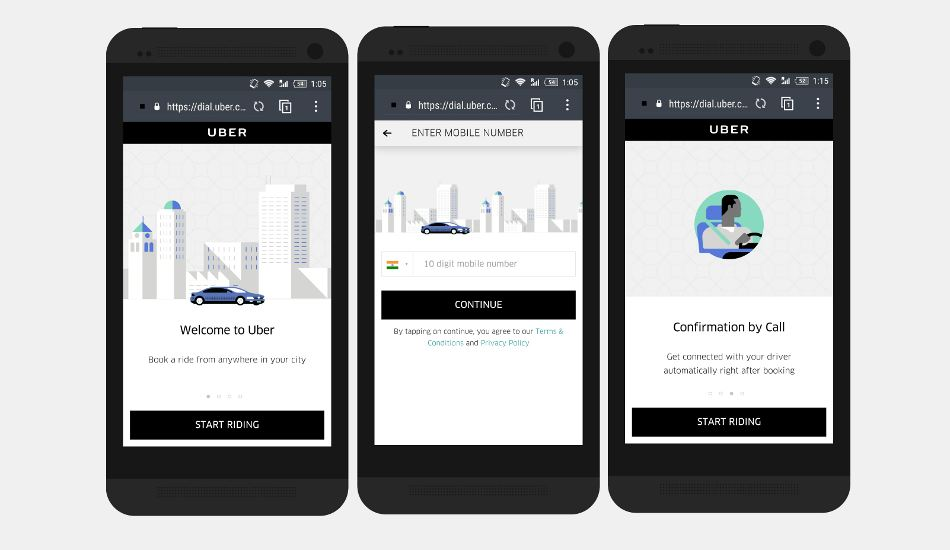
\includegraphics[scale=0.3]{uber1.jpg}
\caption{ثبت نام در اوبر، عکس از themobileindian.com}
\label{fig: uber1}
\end{figure}

\begin{itemize}
\item
قابلیت رزرو یک سرویس تاکسی:  مبدا و مقصد را وارد کرده و به کاربر انواع سرویس‌ها و مبلغ آن‌ها را پیشنهاد می‌دهد، این موارد در شکل \ref{fig: uber2} نمایش داده شده است. رانندگان نزدیک‌‌تر نیز اطلاعات سفر کاربران را دریافت می‌کنند و آن را قبول یا رد می‌کنند.
\end{itemize}

\begin{figure}[htb]
\centering
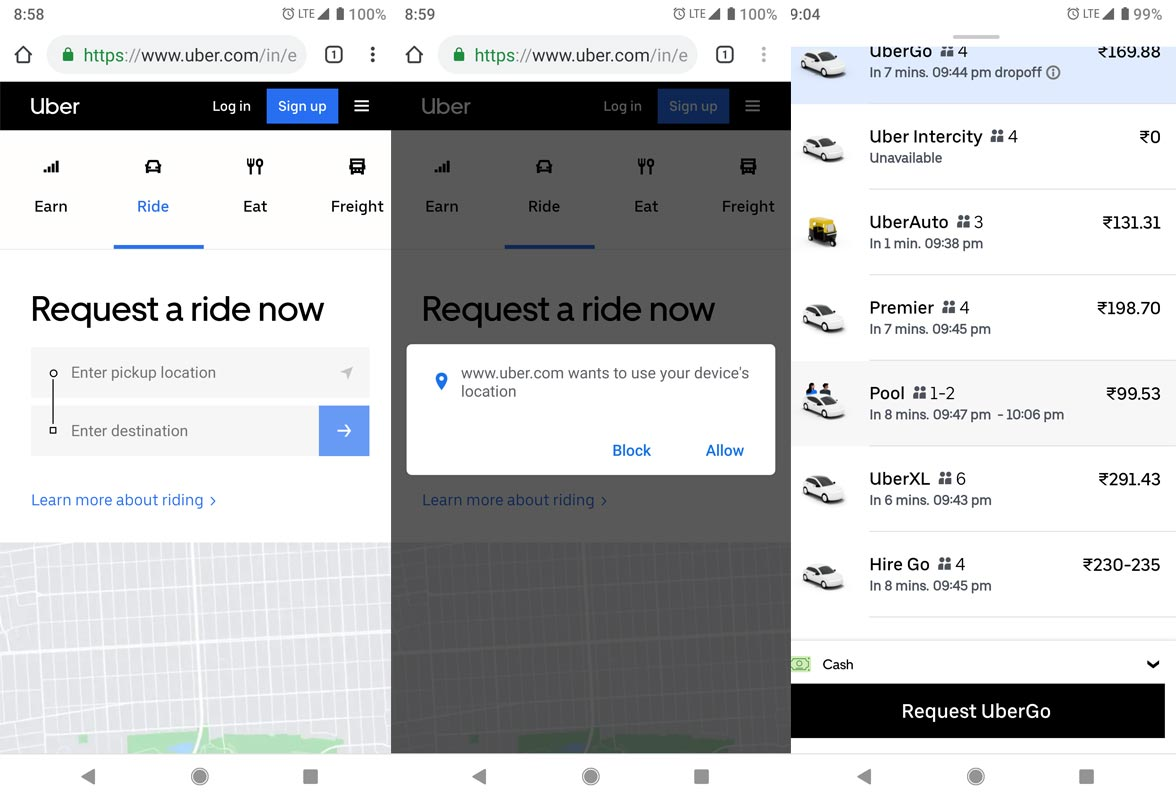
\includegraphics[scale=0.2]{uber2.jpg}
\caption{رزرو تاکسی در اوبر، عکس از  androidinfotech.com}
\label{fig: uber2}
\end{figure}

\begin{itemize}
\item 
دسترسی به موقعیت جغرافیایی و پیدا کردن آن بر روی نقشه در تمامی دستگاه‌های پشتیبانی شده 
\item
نشان دادن نقشه مسیر هم به کاربر و هم به راننده و راهنماییی گام به گام
\item
فرستادن پوش‌نوتیفیکیشن مواقعی که رارننده ای درخواست را اکسپت می‌کند یا به نزدیکی محل می‌رسد یا به هر دلیلی سفر لغو می‌شود.
\item
محاسبه قیمت دقیق بر اساس مبدا و مقصد و ساعت حرکت و نوع ماشین
\item 
قابلیت اشتراک سفر و مسیر خود با دیگران و دنبال کردن در زمان واقعی
\item
قابلیت اضافه کردن نقاط توقف در مسیر 
\item
استفاده از سرویس‌های متنوع پرداخت نظیر paypal ، credit card و ...
\item 
قابلیت برنامه‌ریزی سفر تا ۳۰ روز مانده 
\item 
امکان همگام‌سازی تقویم قرارهای ملاقات با برنامه 
\end{itemize}



\subsection{نیازهای عملکردی \lr{MyWay}}

طبق مستندات \cite{myway_req}برای MyWay می‌توان 100 نیازمندی عملکردی بیان کرد که این نیازمندی‌ها را می‌توان در ۴ دسته کلی زیر طبقه بندی کرد

\begin{itemize}
\item
برنامه‌ریزی سفر و دنبال کردن \footnote{Tracking}
\item 
خدمات تحرک\footnote{Mobility} و آگاهی از منابع
\item 
نمایه کردن \footnote{Profiling} کاربران 
\item 
مدیریت سیستم
\end{itemize} 


از مهمترین نیازمندی‌های این برنامه نیز می‌توان به موارد زیر اشاره کرد:
\begin{itemize}
\item
برنامه‌ریزی سفر
\item
رزرو یک سرویس
\item 
اطلاعات شهر 
\item
نمایه کردن کاربر 
\end{itemize}

در شکل \ref{fig: myway} تعدادی از صفحات نسخه موبایل نمایش داده شده است.
\begin{figure}[htb]
\centering
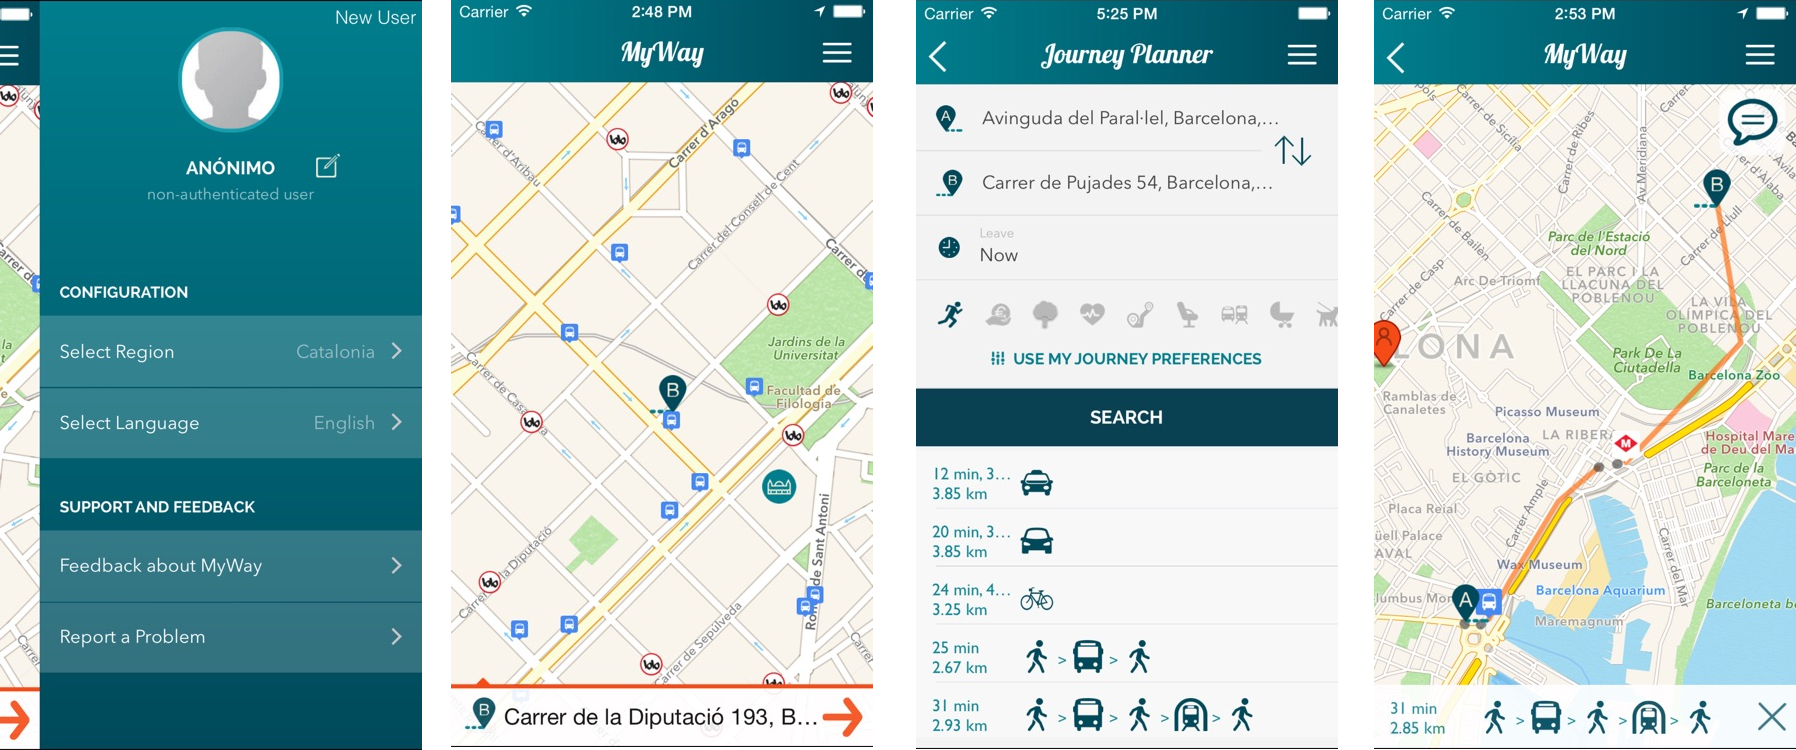
\includegraphics[scale=0.4]{myway.png}
\caption{نمایی از نسخه موبایل اپ Myway تصویر از appadvice.com}
\label{fig: myway}
\end{figure}
از آنجا که نوشتن ریز جزئیات نیازمندی‌های عملکردی هدف این گزارش نیست بنابراین ۴ دسته کلی نیازهای عملکردی را به ۱۴ دسته تقسیم می‌کنیم و آن ۱۴ دسته را همراه با توضیحات گزارش می‌کنیم. 

برنامه‌ریزی سفر و دنبال کردن:
\begin{itemize}
\item
برنامه‌ریزی سفر: نیاز است که کاربر با استفاده از موقعیت مکانی خود، آدرس‌ها، انتخاب نقطه بر روی نقشه، نقاط مورد علاقه یک سفر را برنامه‌ریزی کند و برنامه نیز مسیری بین مبدا و مقصد پیشنهاد دهد و اطلاعات ترافیک را بازتاب دهد و  آن سفر را به پروفایل کاربر اضافه کند و ...
\item 
رزرو کردن یک سرویس: رزو کردن تاکسی، قطار، اتوبوس، اسکوتر، جای پارک 
\item
دنبال کردن یک سفر: دوباره فیدبک‌دهی و محاسبه به کاربر در رابطه با سفر با استفاده از دنبال کردن آن با GPS
\item
فیدبک‌دهی آنلاین از شرایط جاده و محدودیت‌ها
\item
فیدبک دادن به سفر: کاربر می‌تواند فیدبک خود را ارائه دهد.
\end{itemize}

خدمات تحرک و آگاهی از منابع: 
\begin{itemize}
\item
اطلاعات شهر: ذخیره نقاط مورد علافه در شهر و اطلاعات دادن در مورد رستوران‌ها و ارزیابی‌آن‌ها و سرویس‌های زمان‌بندی شده تحرک و اطلاعات در مورد توزیع آن‌ها و ...
\item
فیدبک دادن به Myway در مورد سرویس‌ها
\end{itemize}

نمایه کردن کاربر: 
\begin{itemize}
\item
نمایه کاربر: اضافه کردن اطلاعات عمومی در نمایه کارب رو تغییر آن‌ها، علایق و ترجیحات و ...
\item 
گروه کردن کاربران: بیشتر برای اشتراک‌گذاری خودرو استفاده می‌شود و کاربر می‌تواند یک جامعه اشتراک‌گذاری خودرو درست کند و به آن اضافه و حذف شود و با افراد آن جامعه برنامه سفر خود را به اشتراک بگذارد.
\end{itemize}

مدیریت سیستم:
\begin{itemize}
\item
تحلیل: جمع‌اوری تاریخچه‌ها و انجام عملیات‌های آماری و تحلیل داده‌ها 
\item
احراز هویت کاربر: تعیین نقش و احراز هویت کاربر با استفاده از سیستم احراز هویت
\item 
مدیریت داده: مدیریت شهر‌ها و تنظیمات و تغییر داده ها توسط ادمین‌های Myway
\item 
درگاه برای اپراتور‌های سرویس‌ها
\end{itemize}


\section{اشتراک خودرو و حمل‌و‌نقل درون شهری}
در سال های اخیر دغدغه های اقتصادی،‌زیست محیطی و اجتماعی جوامع را به سمت استفاده مشترک از منابع در دسترس سوق داده است؛صنعت حمل‌و‌نقل نیز از این قاعده مستثنا نبوده و در جهت استفاده مشترک از زیرساخت های موجود گام‌های موثری را برداشته است.

اشتراک خودرو\LTRfootnote{Car Pooling} به معنی به اشتراک گذاشتن خودرو توسط افراد در سفر هایی با مقاصد نزدیک به هم است و در نتیجه سبب می شود تا افراد کمتری برای رفتن به مقاصد خود از خودرو های شخصی استفاده کنند.

با استفاده بیشتر از یک فرد از وسیله نقلیه، هزینه های سفر هر فرد نظیر  هزینه های سوخت، عوارض رانندگی و استرس رانندگی کاهش خواهد یافت.

رانندگان و مسافران سفرها را از طریق یکی از چندین رسانه موجود ارائه می دهند و جستجو می کنند. آنها پس از یافتن افراد با سفر های مشابه با یکدیگر تماس می گیرند تا جزئیات سفر را ترتیب دهند. هزینه ها،‌نقاط ملاقات و سایر جزئیات مانند فضای وسایل اضافه همراه افراد نیز از پیش توافق شده است.‌‌سپس افراد طبق برنامه ریزی از پیش انجام شده با یکدیگر ملاقات نموده و سفر را انجام می دهند.

هم اکنون استارت آپ های زیادی در زمینه ی اشتراک گذاری خودرو در سرتاسر دنیا شروع به فعالیت کرده اند که می توانیم برای مثال از \lr{Waze Car} ، \lr{BlaBla Car} و \lr{Ride Connect} نام ببریم.

از آنجا که استفاده از اشتراک خودرو تعداد خودر‌و‌های مورد نیاز مسافران را کاهش می دهد ، اغلب با مزایای متعددی در جامعه همراه است از جمله: 
\begin{itemize}
\item
کاهش در مصرف انرژی و انتشار گازهای گلخانه ای
\item
کاهش ترافیک سطح شهری
\item
کاهش تقاضای زیرساخت پارکینگ
\end{itemize}

\subsection{نیازهای عملکردی \lr{Waze Carpool}}
اشتراک‌گذاری خودرو به دو صورت در شرکت waze انجام می‌شود. یک آن که در خود اپلکیشن اصلی waze یک گزینه جدا برای اشتراک‌گذاری خودرو وجود دارد. دو، برنامه مجزا این شرکت برای اشتراک‌گذاری خودرو است \cite{waze_carpool} .

هر یک از افراد می‌توانند در نقش راننده یا مسافر ظاهر شوند. برای مسافر تنها کافی است زمان اشتراک‌گذاری خودرو را تنظیم کنند، مشاهده کنند که چه کسی در آن زمان رانندگی می‌کند و از او درخواست عضویت کنند و سپس با یکدیگر تایید کنند.
برای رانندگی نیز کافیست که زمان، تعداد صندلی‌ها و مسیر خود را مشخص کنید از مسافران دعوت کنید و اشتراک‌گذاری خودرو را شروع کنید. نحوه درخواست از راننده برای برنامه موبایل در تصویر \ref{fig: waze1} نمایش داده شده است.


\begin{figure}[hbt]
\centering
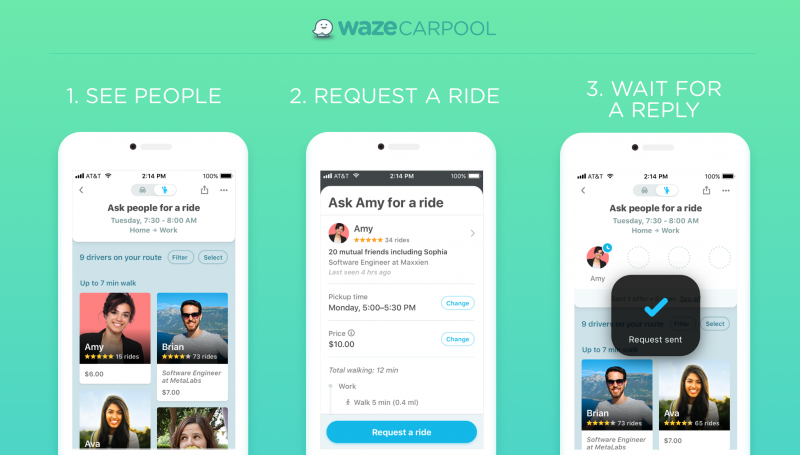
\includegraphics[scale=0.5]{waze1.png}
\caption{درخواست خودرو برای هم‌اشتراک‌گذاری، عکس از sourceWaze}
\label{fig: waze1}
\end{figure}

از مهمترین نیازمندی‌های این برنامه می‌توان به موارد زیر اشاره کرد:

\begin{itemize}
\item
ثبت نام و ورود به برنامه
\item
وارد کردن اطلاعات در نمایه و تغییر ان‌ها
\item
تنظیم زمان اشتراک گذاری خودرو و مسیر برای راننده و مسافر
\item
درخواست به رانندگان 
\item
مشاهده درخواست مسافران و قبول و رد ان‌ها 
\item
چت و گرفتن تایید بین راننده و مسافر
\item 
پرداخت با روش‌های مختلف
\item
تایید رانندگان با سرویس‌های ثالث 
\end{itemize}


\section{پارکنیگ های عمومی و حمل‌و‌نقل درون شهری}
برای افرادی که در شهر های بزرگ زندگی می کنند یافتن پارکینگ مقرون به صرفه می تواند یک چالش باشد؛ طی تحقیق که توسط IBM انجام شد محققان به این واقعیت پی ردند که نزدیک به  30٪ از ترافیك شهر به رانندگانی كه بدنبال پارکینگ هستند، نسبت داده می شود. خوشبختانه، برنامه های مختلفی برای کمک به افراد در پیدا کردن و مقایسه نقاط پارک مناسب وجود دارند که برخی از آن ها حتی امکان رزرو پارکینگ را در اختیار کاربران خود قرار می دهند.

از جمله برنامه هایی که در زمینه‌ی پارکنیگ های درون شهری در آمریکا فعالیت می کنند می توان به \lr{Best Parking} و یا ParkWhiz اشاره کرد.


\subsection{نیازهای عملکردی \lr{ParkWhiz}}
از مهمترین نیازمندی‌های این برنامه می‌توان به موارد زیر اشاره کرد:

\begin{itemize}
\item
ثبت نام و ورود به برنامه
\item
وارد کردن اطلاعات در نمایه و تغییر ان‌ها
\item
پیدا کردن پارکینگ‌ها برای الان یا برای بعد ، مقایسه قیمت آن‌ها و فاصله آن‌ها تا مقصد اصلی کاربر
\item
رزرو کردن پارکینگ در ساعت دلخواه 
\item
اتصال به سرویس‌های مسیریابی برای رسیدن به پارکینگ
\item
پرداخت راحت بوسیله کارت‌های اعتباری یا دروازه‌های پرداخت‌ دیجیتال
\item
خروجی گرفتن از رزرو انجام شده و مشاهده اطلاعات رزرو
\item
پنل ادمین برای مدیریت پارکینگ و ایجاد تغییرات و  عملیات‌های مدیریت و گزارش گیری 
\end{itemize}

در شکل \ref{fig: parkwhiz1} نحوه پیدا کردن پارکینگ و مقایسه آن‌ها بر اساس قیمت و فاصله نمایش داده شده است.



\begin{figure}[htb]
\centering
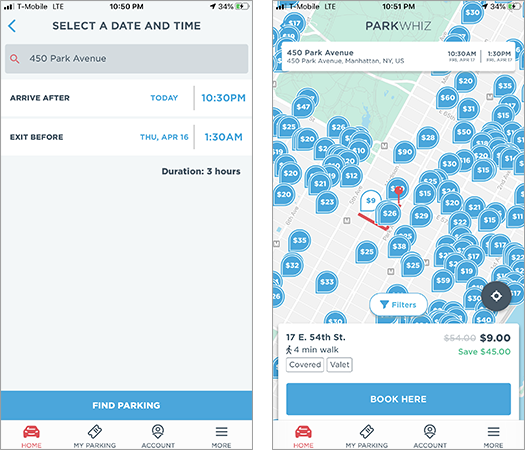
\includegraphics[scale=0.5]{parkwhiz1.png}
\caption{جستجو پارکینگ و مقایسه، عکس از \cite{parkwhiz_ux}}
\label{fig: parkwhiz1}
\end{figure}
















